%% Version 4.3.2, 25 August 2014
%
%%%%%%%%%%%%%%%%%%%%%%%%%%%%%%%%%%%%%%%%%%%%%%%%%%%%%%%%%%%%%%%%%%%%%%
% Template.tex --  LaTeX-based template for submissions to the 
% American Meteorological Society
%
% Template developed by Amy Hendrickson, 2013, TeXnology Inc., 
% amyh@texnology.com, http://www.texnology.com
% following earlier work by Brian Papa, American Meteorological Society
%
% Email questions to latex@ametsoc.org.
%
%%%%%%%%%%%%%%%%%%%%%%%%%%%%%%%%%%%%%%%%%%%%%%%%%%%%%%%%%%%%%%%%%%%%%
% PREAMBLE
%%%%%%%%%%%%%%%%%%%%%%%%%%%%%%%%%%%%%%%%%%%%%%%%%%%%%%%%%%%%%%%%%%%%%

%% Start with one of the following:
% DOUBLE-SPACED VERSION FOR SUBMISSION TO THE AMS
\documentclass{ametsoc}

% TWO-COLUMN JOURNAL PAGE LAYOUT---FOR AUTHOR USE ONLY
% \documentclass[twocol]{ametsoc}

%%%%%%%%%%%%%%%%%%%%%%%%%%%%%%%%
%%% To be entered only if twocol option is used

\journal{jas}

%  Please choose a journal abbreviation to use above from the following list:
% 
%   jamc     (Journal of Applied Meteorology and Climatology)
%   jtech     (Journal of Atmospheric and Oceanic Technology)
%   jhm      (Journal of Hydrometeorology)
%   jpo     (Journal of Physical Oceanography)
%   jas      (Journal of Atmospheric Sciences)	
%   jcli      (Journal of Climate)
%   mwr      (Monthly Weather Review)
%   wcas      (Weather, Climate, and Society)
%   waf       (Weather and Forecasting)
%   bams (Bulletin of the American Meteorological Society)
%   ei    (Earth Interactions)

%%%%%%%%%%%%%%%%%%%%%%%%%%%%%%%%
%Citations should be of the form ``author year''  not ``author, year''
\bibpunct{(}{)}{;}{a}{}{,}

%%%%%%%%%%%%%%%%%%%%%%%%%%%%%%%%

%%% To be entered by author:

%% May use \\ to break lines in title:

\title{Tropopause Evolution in a Rapidly Intensifying Tropical Cyclone: A Static Stability Budget Analysis}

%%% Enter authors' names, as you see in this example:
%%% Use \correspondingauthor{} and \thanks{Current Affiliation:...}
%%% immediately following the appropriate author.
%%%
%%% Note that the \correspondingauthor{} command is NECESSARY.
%%% The \thanks{} commands are OPTIONAL.

    %\authors{Author One\correspondingauthor{Author One, 
    % American Meteorological Society, 
    % 45 Beacon St., Boston, MA 02108.}
% and Author Two\thanks{Current affiliation: American Meteorological Society, 
    % 45 Beacon St., Boston, MA 02108.}}

\authors{Patrick Duran\correspondingauthor{Department of Atmospheric and Environmental Sciences, University at Albany, State University of New York, 1400 Washington Avenue, Albany, NY.} and John Molinari}

%% Follow this form:
    % \affiliation{American Meteorological Society, 
    % Boston, Massachusetts.}

\affiliation{University at Albany, State University of New York,
Albany, NY}

%% Follow this form:
    %\email{latex@ametsoc.org}

\email{pduran2008@gmail.com}

%% If appropriate, add additional authors, different affiliations:
    %\extraauthor{Extra Author}
    %\extraaffil{Affiliation, City, State/Province, Country}

%\extraauthor{}
%\extraaffil{}

%% May repeat for a additional authors/affiliations:

%\extraauthor{}
%\extraaffil{}

%%%%%%%%%%%%%%%%%%%%%%%%%%%%%%%%%%%%%%%%%%%%%%%%%%%%%%%%%%%%%%%%%%%%%
% ABSTRACT
%
% Enter your abstract here
% Abstracts should not exceed 250 words in length!
%
% For BAMS authors only: If your article requires a Capsule Summary, please place the capsule text at the end of your abstract
% and identify it as the capsule. Example: This is the end of the abstract. (Capsule Summary) This is the capsule summary. 

\abstract{Enter the text of your abstract here.}

\begin{document}

%% Necessary!
\maketitle


%%%%%%%%%%%%%%%%%%%%%%%%%%%%%%%%%%%%%%%%%%%%%%%%%%%%%%%%%%%%%%%%%%%%%
% MAIN BODY OF PAPER
%%%%%%%%%%%%%%%%%%%%%%%%%%%%%%%%%%%%%%%%%%%%%%%%%%%%%%%%%%%%%%%%%%%%%
%

%% In all cases, if there is only one entry of this type within
%% the higher level heading, use the star form: 
%%
 \section{Introduction}

There will be a whole bunch of papers cited here...

 \section{Model Setup}

Put description of Fig.~\ref{fig:vmax+pmin} in this section. 

Don't forget to mention 1-2-1 smoother.

 \section{Budget Computation}

Add details of budget computation here...

 \section{Results}

 \subsection{Static stability evolution}

The average N\textsuperscript{2} over the first day of the simulation (Fig.~\ref{fig:n2-24hr-avgs}a) indicates the presence of a static stability maximum about 400 m above the cold-point tropopause.
This lower-stratospheric stable layer had begun to erode during the initial spin-up period, with the maximum destabilitzation occurring at the innermost radii.
This decrease in static stability continued into the second day of the simulation (Fig.~\ref{fig:n2-24hr-avgs}b) as the storm intensified to hurricane strength (Fig.~\ref{fig:vmax+pmin}).
Destabilization was particularly pronounced over the developing eye, where the time-mean cold-point tropopause height increased by up to 400 m compared to the previous day.
Over the developing eyewall and outer rainband regions, meanwhile, the tropopause height remained nearly constant.
During the third day of the simulation (Fig.~\ref{fig:n2-24hr-avgs}c), static stability over the eye continued to decrease, and the cold-point tropopause height rose to 18.3 km at the storm center.
The tropopause sloped sharply downward over the innermost radii, reaching the 16.4-km level near the 50-km radius.
This local minimum in tropopause height corresponded to the eyewall region, where upper-tropospheric static stability increased during this time period.
Outside of the eyewall region, static stability began to increase in the layer immediately overlying the cold-point tropopause.
This stable layer sloped upward with radius, which corresponded to an upward-sloping tropopause radially outside of the eywall region.
Over the next 24 hours (Fig.~\ref{fig:n2-24hr-avgs}d), as the storm's maximum 10-m wind speed leveled off near 80 m s\textsuperscript{-1} (Fig.~\ref{fig:vmax+pmin}), the upper-tropospheric static stability within the eyewall region continued to strengthen, along with the static stability within the lower stratosphere radially outside of the eyewall.
As the stable layer strengthened, its altitude rose slightly, which corresponded to a slight increase in tropopause height outside of the eyewall during this period.
Within the upper troposphere radially outside of the eyewall, meanwhile, static stability decreased such that it was nearly neutral in a thin layer between the 120- and 150-km radii.
The eye region likewise continued to destabilize, and the cold-point tropopause height increased to a level above 18.5 km.
This static stability evolution closely follows that observed in Hurricane Patricia (2015; \citeauthor{Duran+Molinari2018} \citeyear{Duran+Molinari2018}).

 \subsection{Static stability budget analysis}

The left column of Fig.~\ref{fig:modbudres} depicts 24-hour changes in N\textsuperscript{2} over each of the four days of the simulation. 
These represent bulk changes computed by subtracting the instantaneous N\textsuperscript{2} at the initial time from the instantaneous N\textsuperscript{2} at the final time. 
The middle column of Fig.~\ref{fig:modbudres} represents the change in N\textsuperscript{2} computed using Eq. XXX and the method described in Section 3. 
The residual between these two computations (Fig.~\ref{fig:modbudres}, right column) is much smaller than the change in N\textsuperscript{2}, meaning that the budget peforms well within the analysis domain.

To determine which of the budget terms are most important, a time series of the contribution of each of the budget terms in Eq. XXX to the tropopause-layer static stability tendency is plotted in Fig. \ref{fig:avgbudterms}.
For this figure, each of the budget terms is computed using the method described in Section 3, except with 1-hour averaging intervals instead of 24-hour intervals.
The absolute values of these tendencies are then averaged over the radius-height domain depicted in Fig.~\ref{fig:modbudres} and plotted as a time series\footnote{It will be seeen in subsequent figures that each of the terms contributes both positively and negatively to the N\textsuperscript{2} tendency within the analysis domain. 
Thus, taking an average over the domain tends to wash out the positive and negative contributions.
To circumvent this problem, the absolute value of each of the terms is averaged, yielding a time series of the mean magnitude of each budget term.}. 
Advection (Fig.~\ref{fig:avgbudterms}, red line) plays an important role in the mean tropopause-layer static stability tendency at all times, and vertical turbulence (Fig.~\ref{fig:avgbudterms}, blue line) and radiation (Fig.~\ref{fig:avgbudterms}, dark green line) both become important after 48 hours.
Although the contribution from horizontal turbulence (Fig.~\ref{fig:avgbudterms}, purple line) becomes more important after 72 hours, it is confined to a very small region immediately surrounding the eyewall tangential velocity maximum (not shown), and is negligible throughout the rest of the tropopause layer.
The remaining two processes - microphysics and dissipative heating (Fig.~\ref{fig:avgbudterms}, orange and light green lines, respectively) - lie atop one another near zero.
These time series indicate that, at all times, three budget terms dominate the tropopause-layer static stability tendency: advection, vertical turbulence, and radiation.
Variations in the magnitude and spatial structure of these terms drive the static stability changes depicted in Fig.~\ref{fig:n2-24hr-avgs}; subsequent sections will focus on these variations and what causes them.

\paragraph{0-24 hours}
\paragraph{24-48 hours}
\paragraph{48-72 hours}
\paragraph{72-96 hours}

% text...
% \section{Section title}

%vs

% \section{Section title}
% \subsection{subsection one}
% text...
% \subsection{subsection two}
% \section{Section title}

%%%
% \section{First primary heading}

% \subsection{First secondary heading}

% \subsubsection{First tertiary heading}

% \paragraph{First quaternary heading}

%%%%%%%%%%%%%%%%%%%%%%%%%%%%%%%%%%%%%%%%%%%%%%%%%%%%%%%%%%%%%%%%%%%%%
% ACKNOWLEDGMENTS
%%%%%%%%%%%%%%%%%%%%%%%%%%%%%%%%%%%%%%%%%%%%%%%%%%%%%%%%%%%%%%%%%%%%%
%
\acknowledgments
Start acknowledgments here.

%%%%%%%%%%%%%%%%%%%%%%%%%%%%%%%%%%%%%%%%%%%%%%%%%%%%%%%%%%%%%%%%%%%%%
% APPENDIXES
%%%%%%%%%%%%%%%%%%%%%%%%%%%%%%%%%%%%%%%%%%%%%%%%%%%%%%%%%%%%%%%%%%%%%
%
% Use \appendix if there is only one appendix.
%\appendix

% Use \appendix[A], \appendix}[B], if you have multiple appendixes.
%\appendix[A]

%% Appendix title is necessary! For appendix title:
%\appendixtitle{}

%%% Appendix section numbering (note, skip \section and begin with \subsection)
% \subsection{First primary heading}

% \subsubsection{First secondary heading}

% \paragraph{First tertiary heading}

%% Important!
%\appendcaption{<appendix letter and number>}{<caption>} 
%must be used for figures and tables in appendixes, e.g.,
%

%
% All appendix figures/tables should be placed in order AFTER the main figures/tables, i.e., tables, appendix tables, figures, appendix figures.
%
%%%%%%%%%%%%%%%%%%%%%%%%%%%%%%%%%%%%%%%%%%%%%%%%%%%%%%%%%%%%%%%%%%%%%
% REFERENCES
%%%%%%%%%%%%%%%%%%%%%%%%%%%%%%%%%%%%%%%%%%%%%%%%%%%%%%%%%%%%%%%%%%%%%
% Make your BibTeX bibliography by using these commands:
 \bibliographystyle{ametsoc2014}
 \bibliography{references}

%%%%%%%%%%%%%%%%%%%%%%%%%%%%%%%%%%%%%%%%%%%%%%%%%%%%%%%%%%%%%%%%%%%%%
% TABLES
%%%%%%%%%%%%%%%%%%%%%%%%%%%%%%%%%%%%%%%%%%%%%%%%%%%%%%%%%%%%%%%%%%%%%
%% Enter tables at the end of the document, before figures.
%%
%
%\begin{table}[t]
%\caption{This is a sample table caption and table layout.  Enter as many tables as
%  necessary at the end of your manuscript. Table from Lorenz (1963).}\label{t1}
%\begin{center}
%\begin{tabular}{ccccrrcrc}
%\hline\hline
%$N$ & $X$ & $Y$ & $Z$\\
%\hline
% 0000 & 0000 & 0010 & 0000 \\
% 0005 & 0004 & 0012 & 0000 \\
% 0010 & 0009 & 0020 & 0000 \\
% 0015 & 0016 & 0036 & 0002 \\
% 0020 & 0030 & 0066 & 0007 \\
% 0025 & 0054 & 0115 & 0024 \\
%\hline
%\end{tabular}
%\end{center}
%\end{table}

%%%%%%%%%%%%%%%%%%%%%%%%%%%%%%%%%%%%%%%%%%%%%%%%%%%%%%%%%%%%%%%%%%%%%
% FIGURES
%%%%%%%%%%%%%%%%%%%%%%%%%%%%%%%%%%%%%%%%%%%%%%%%%%%%%%%%%%%%%%%%%%%%%
%% Enter figures at the end of the document, after tables.
%%
%


%FIGURE 1%
\begin{figure}[ht]
\centerline{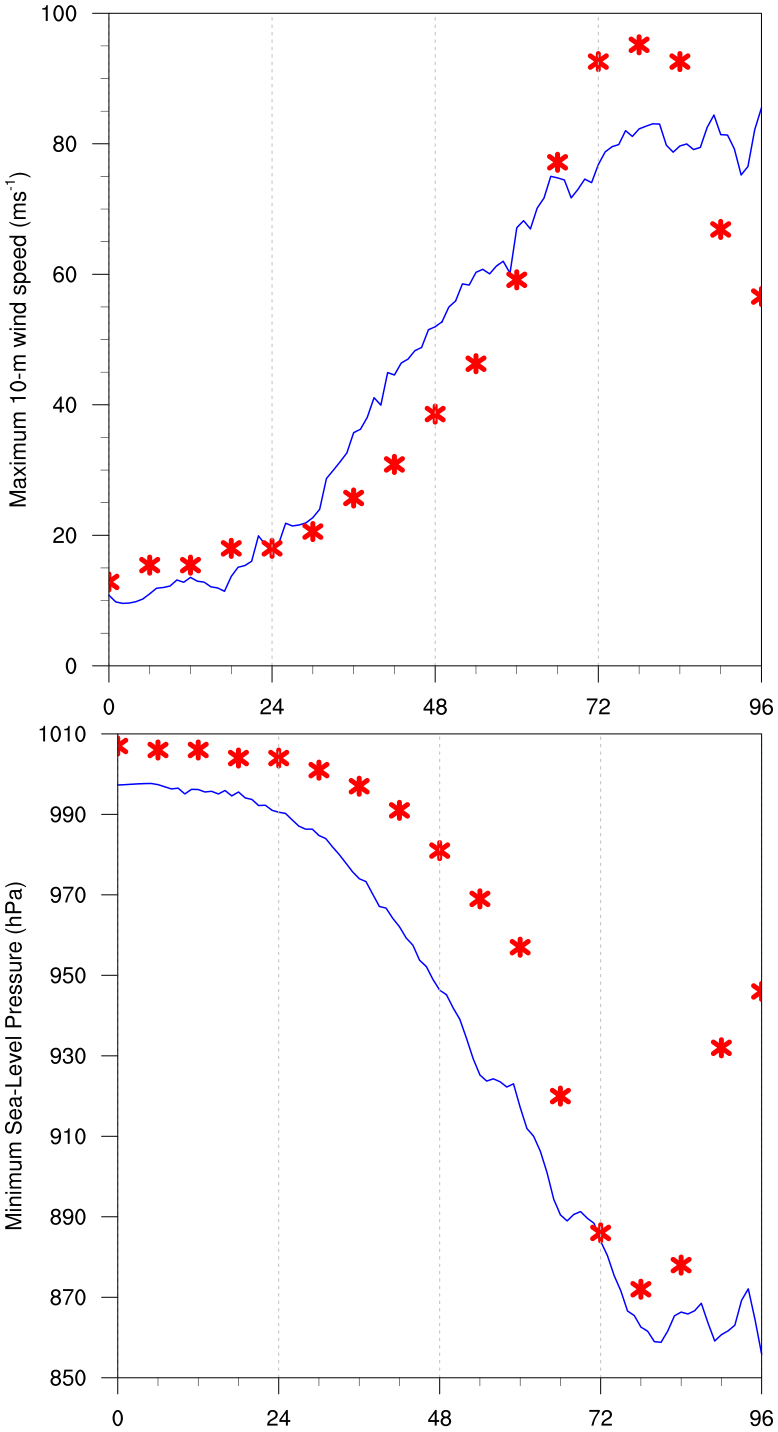
\includegraphics[width=19pc]{figures/fig01_vmax+pmin.png}}
\caption{The maximum 10-m wind speed (top panel; m s\textsuperscript{-2}) and minimum sea-level pressure (bottom panel; hPa) in the simulated storm (blue lines) and from Hurricane Patricia's best track (red stars).}
\label{fig:vmax+pmin}
\end{figure}

%FIGURE 2%
\begin{figure*}[ht]
\centerline{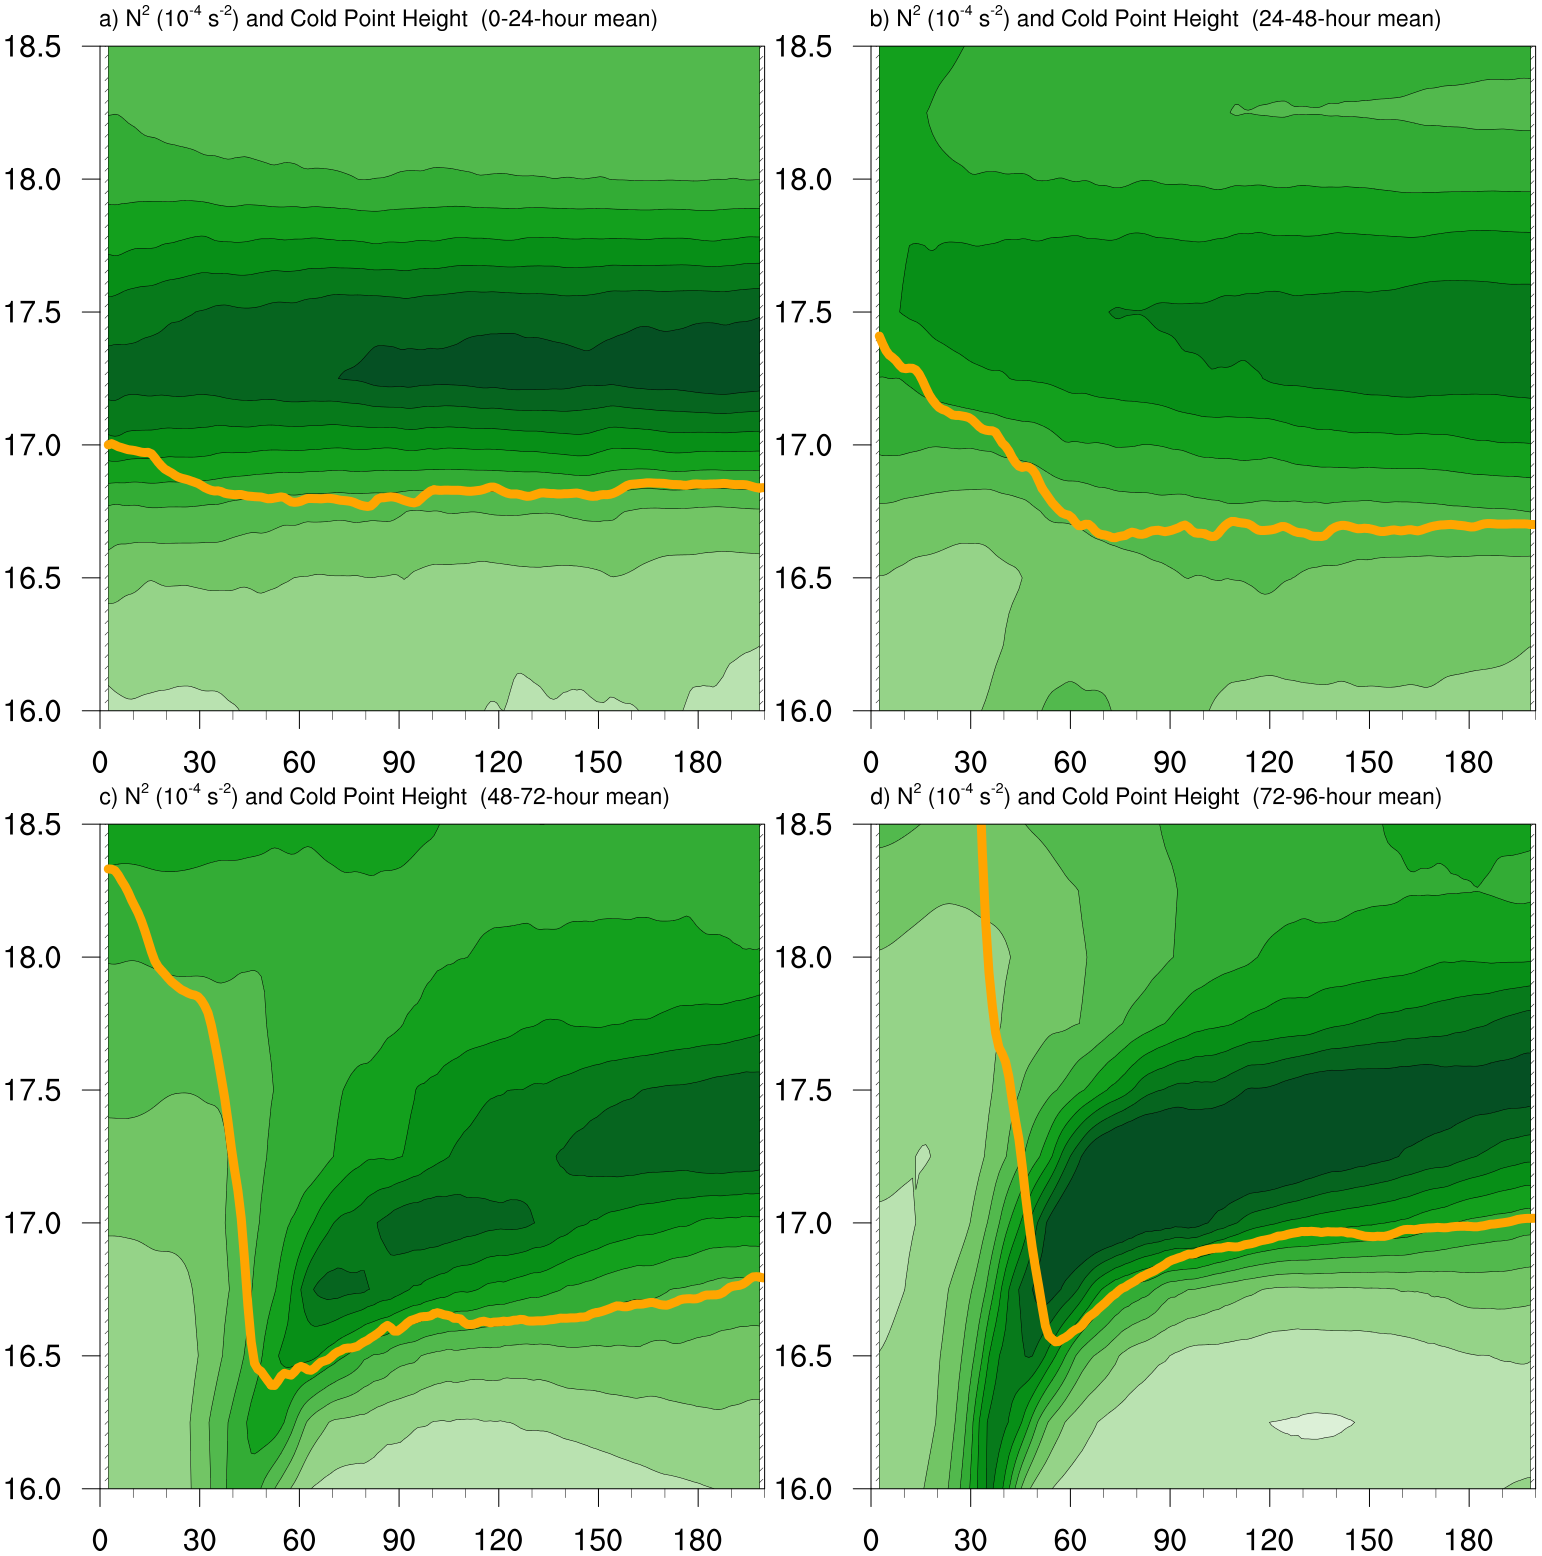
\includegraphics[width=39pc]{figures/fig02_n2-24hr-avgs.png}}
\caption{Twenty-four-hour averages of squared Brunt-V{\"a}is{\"a}l{\"a} frequency (10\textsuperscript{-4} s\textsuperscript{-2}) over the first four days of the simulation. Orange lines represent the cold-point tropopause computed from the mean temperature field over the same time periods.}
\label{fig:n2-24hr-avgs}
\end{figure*}

%FIGURE 3%
\begin{figure*}[ht]
\centerline{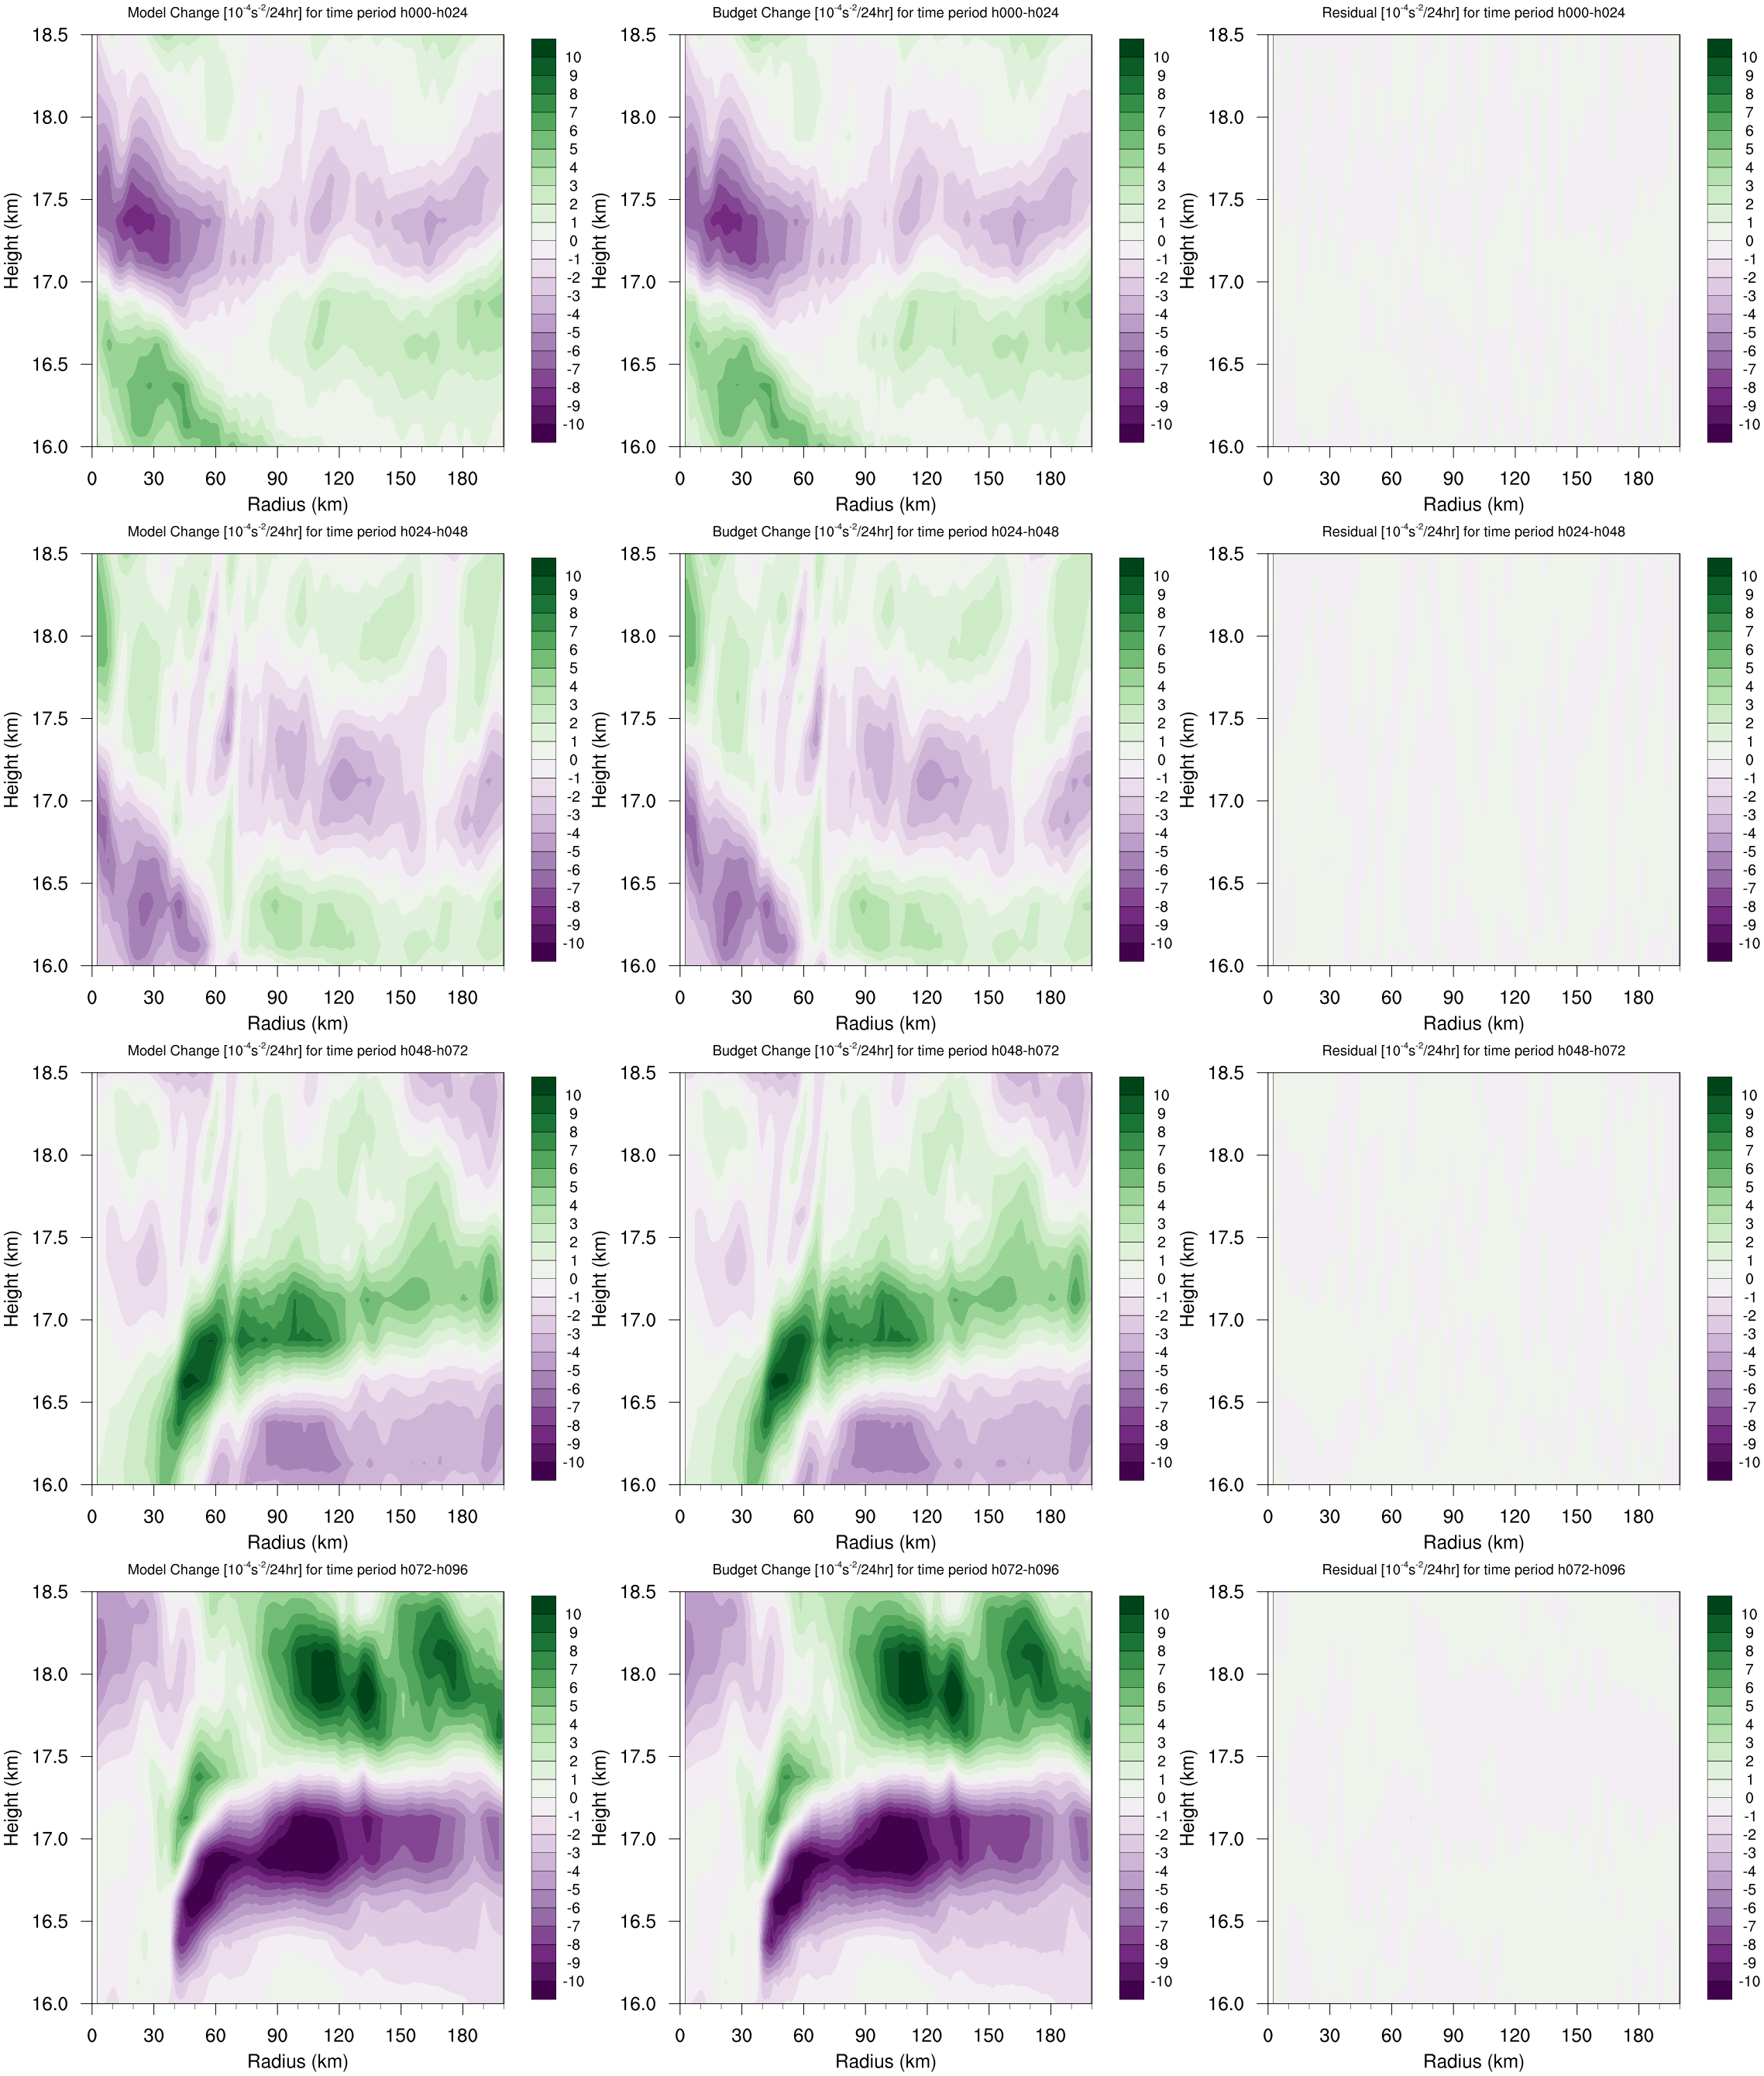
\includegraphics[width=39pc]{figures/fig03_R-Z_mod+bud+res.png}}
\caption{Left panels: Twenty-four-hour changes in squared Brunt-V{\"a}is{\"a}l{\"a} frequency (10\textsuperscript{-4} s\textsuperscript{-2}) over (a) 0-24 hours, (b) 24-48 hours, (c) 48-72 hours, (d) 72-96 hours. Middle Panels: The N\textsuperscript{2} change over the same time periods computed using Eq. XXX. Right Panels: The budget residual over the same time periods, computed by subtracting the budget change (middle column) from the model change (left column).}
\label{fig:modbudres}
\end{figure*}

%FIGURE 4%
\begin{figure}[ht]
\centerline{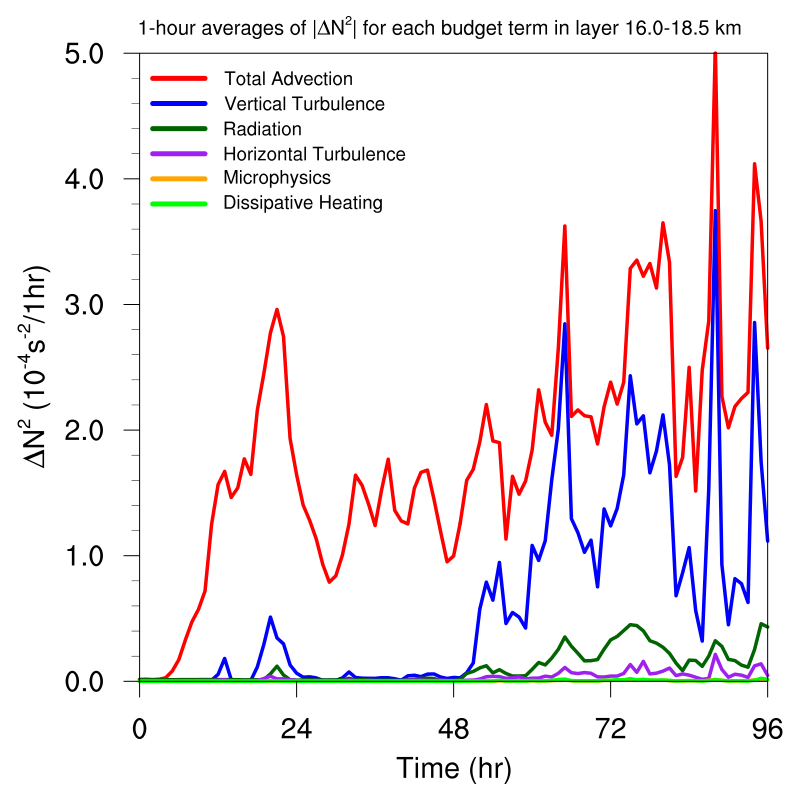
\includegraphics[width=19pc]{figures/fig04_AVG_budterms.png}}
\caption{Time series of the contribution of each of the budget terms to the time tendency of the squared Brunt-V{\"a}is{\"a}l{\"a} frequency (N\textsuperscript{2}; 10\textsuperscript{-4} s\textsuperscript{-2}). For each budget term, the absolute value of the N\textsuperscript{2} tendency is averaged both temporally over 1-hour periods (using output every minute), and spatially within the radius-height domain depicted in Fig.~\ref{fig:modbudres}.}
\label{fig:avgbudterms}
\end{figure}

%FIGURE 5%
\begin{figure*}[ht]
\centerline{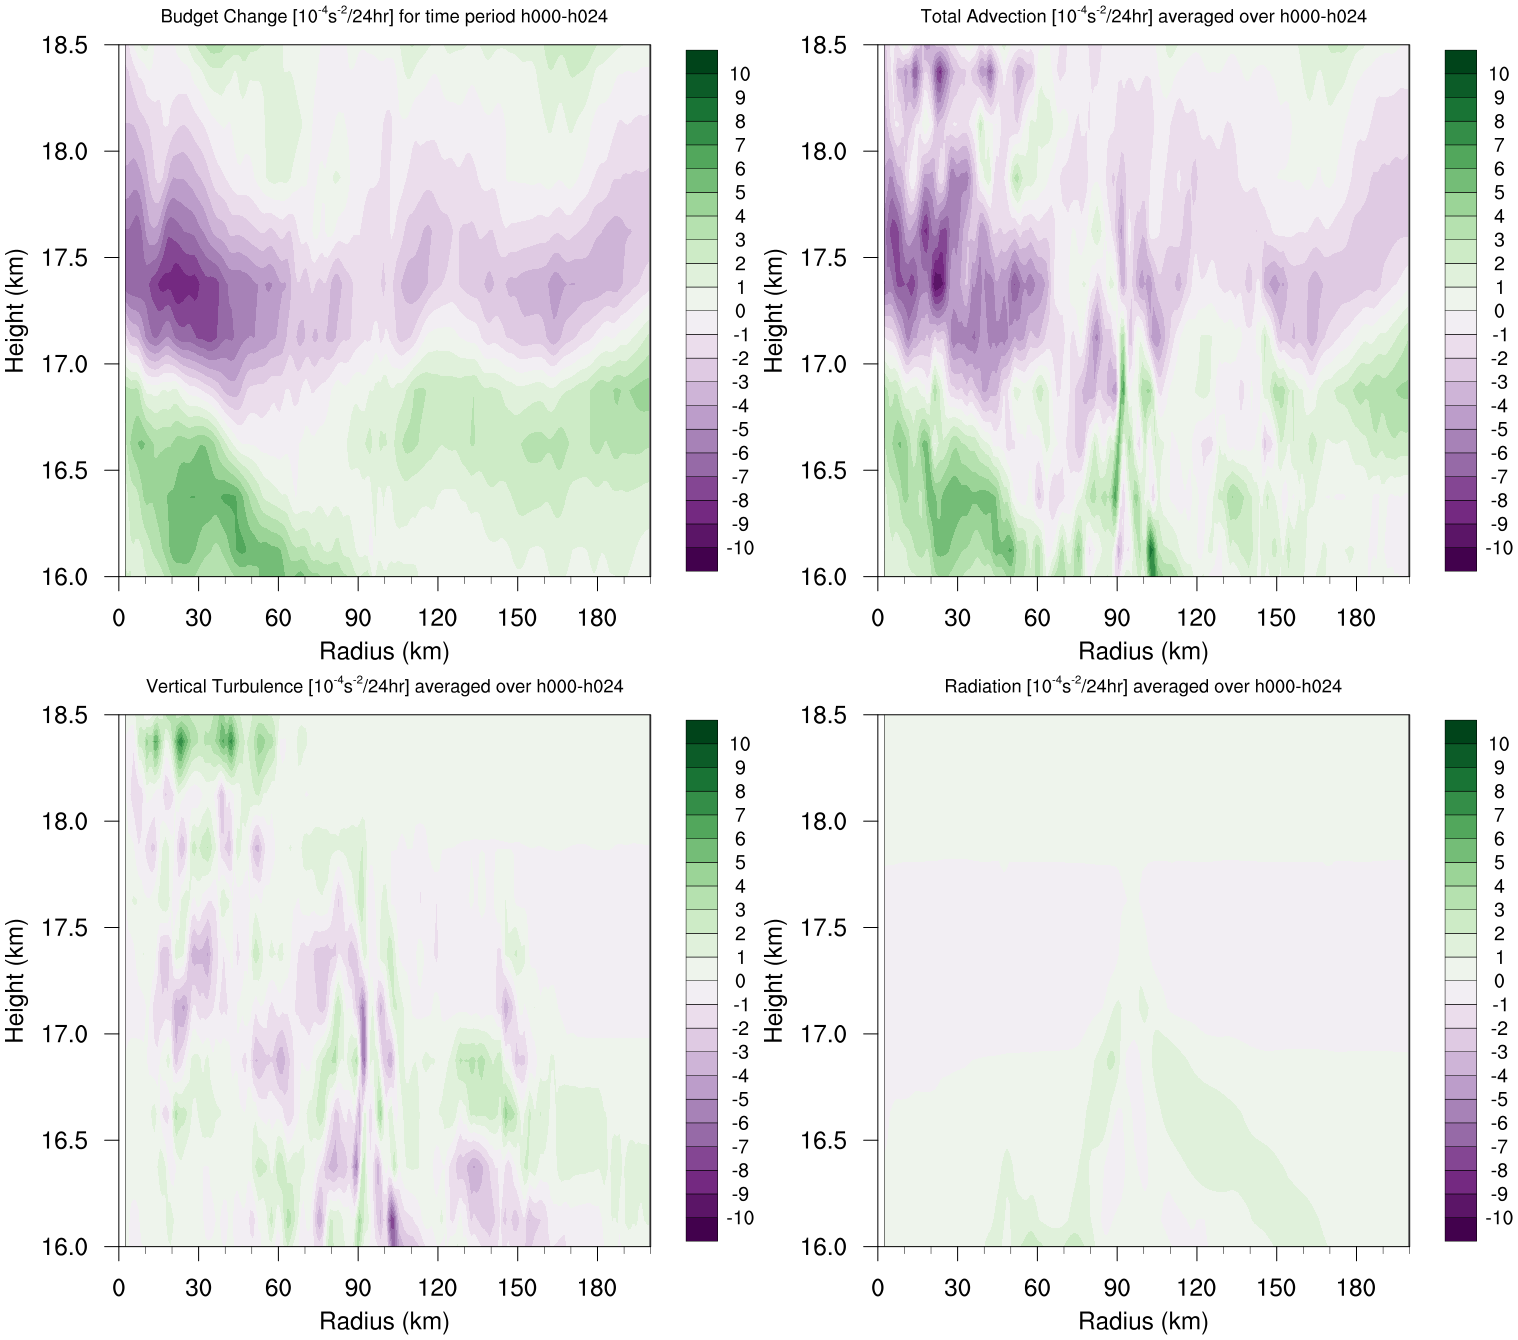
\includegraphics[width=39pc]{figures/fig05_h000-h024-budgetterms.png}}
\caption{}
\label{fig:00-24}
\end{figure*}

%FIGURE 6%
\begin{figure*}[ht]
\centerline{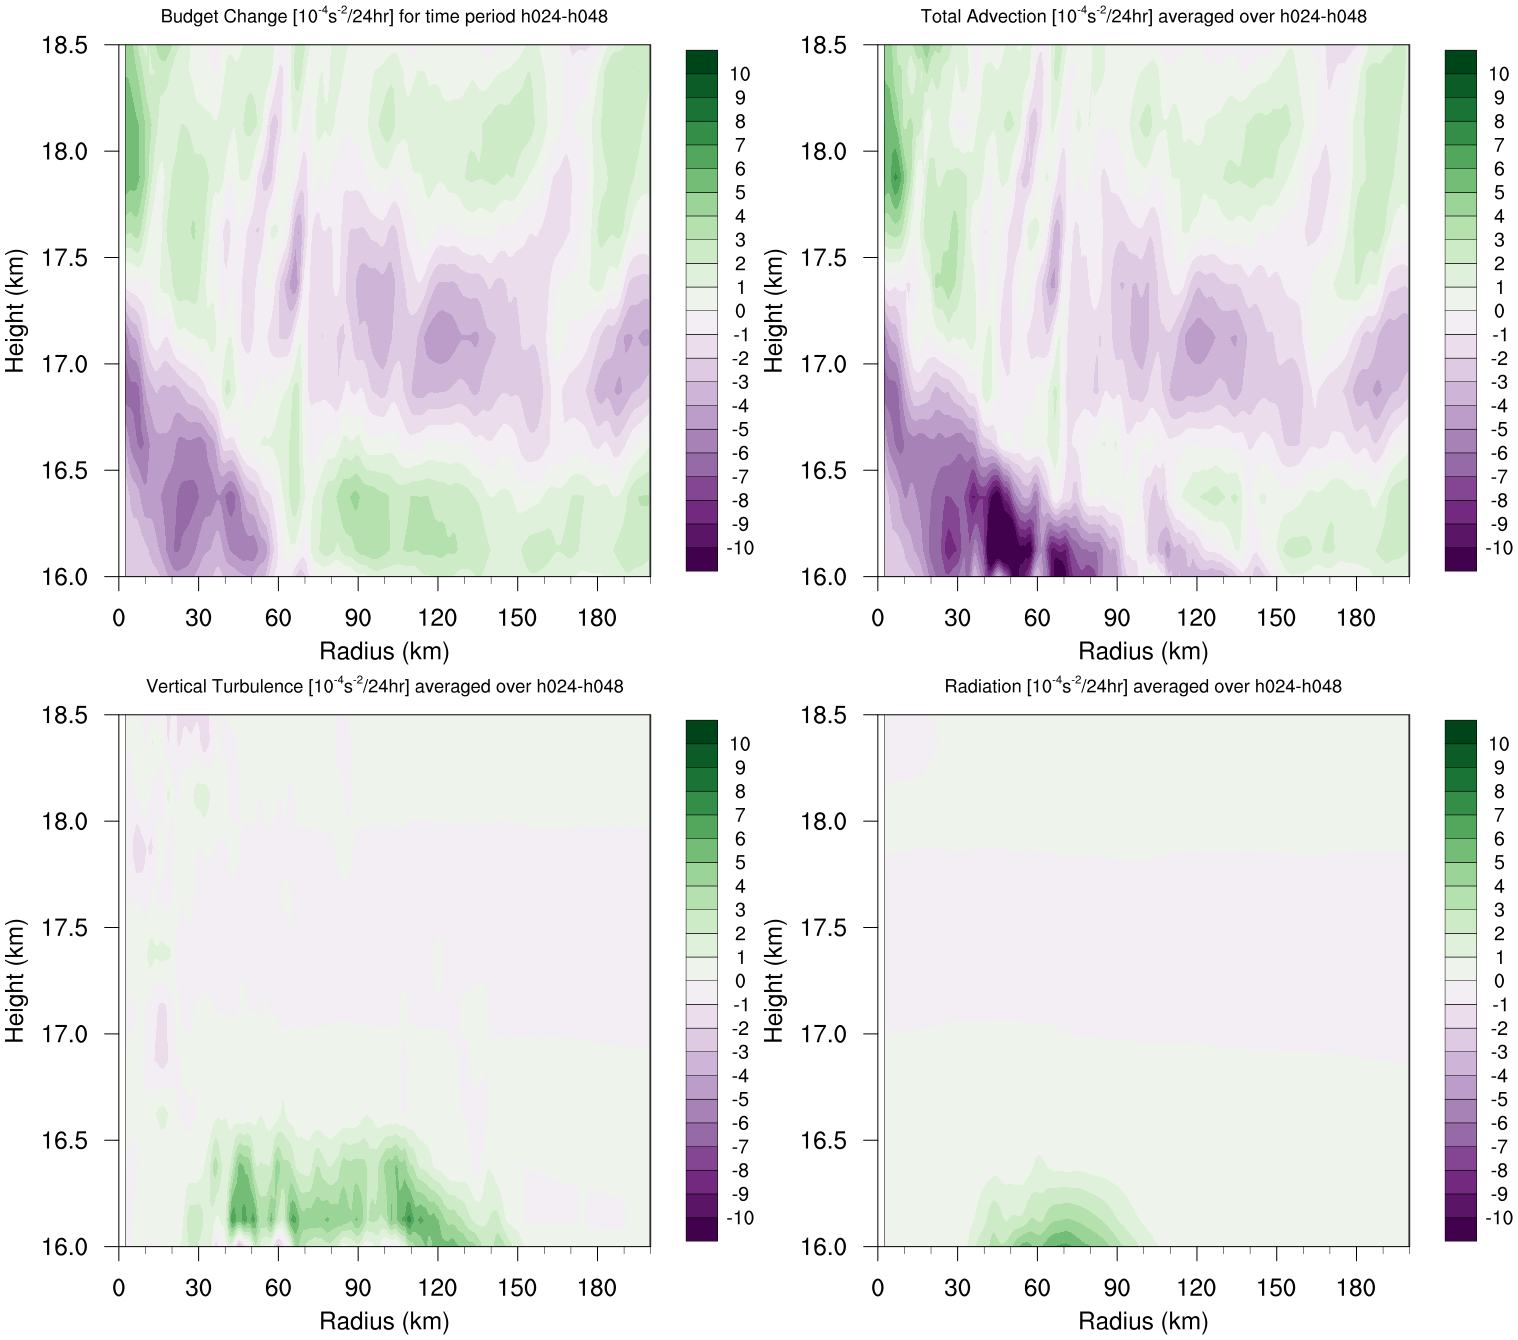
\includegraphics[width=39pc]{figures/fig06_h024-h048-budgetterms.png}}
\caption{}
\label{fig:24-48}
\end{figure*}

%FIGURE 7%
\begin{figure*}[ht]
\centerline{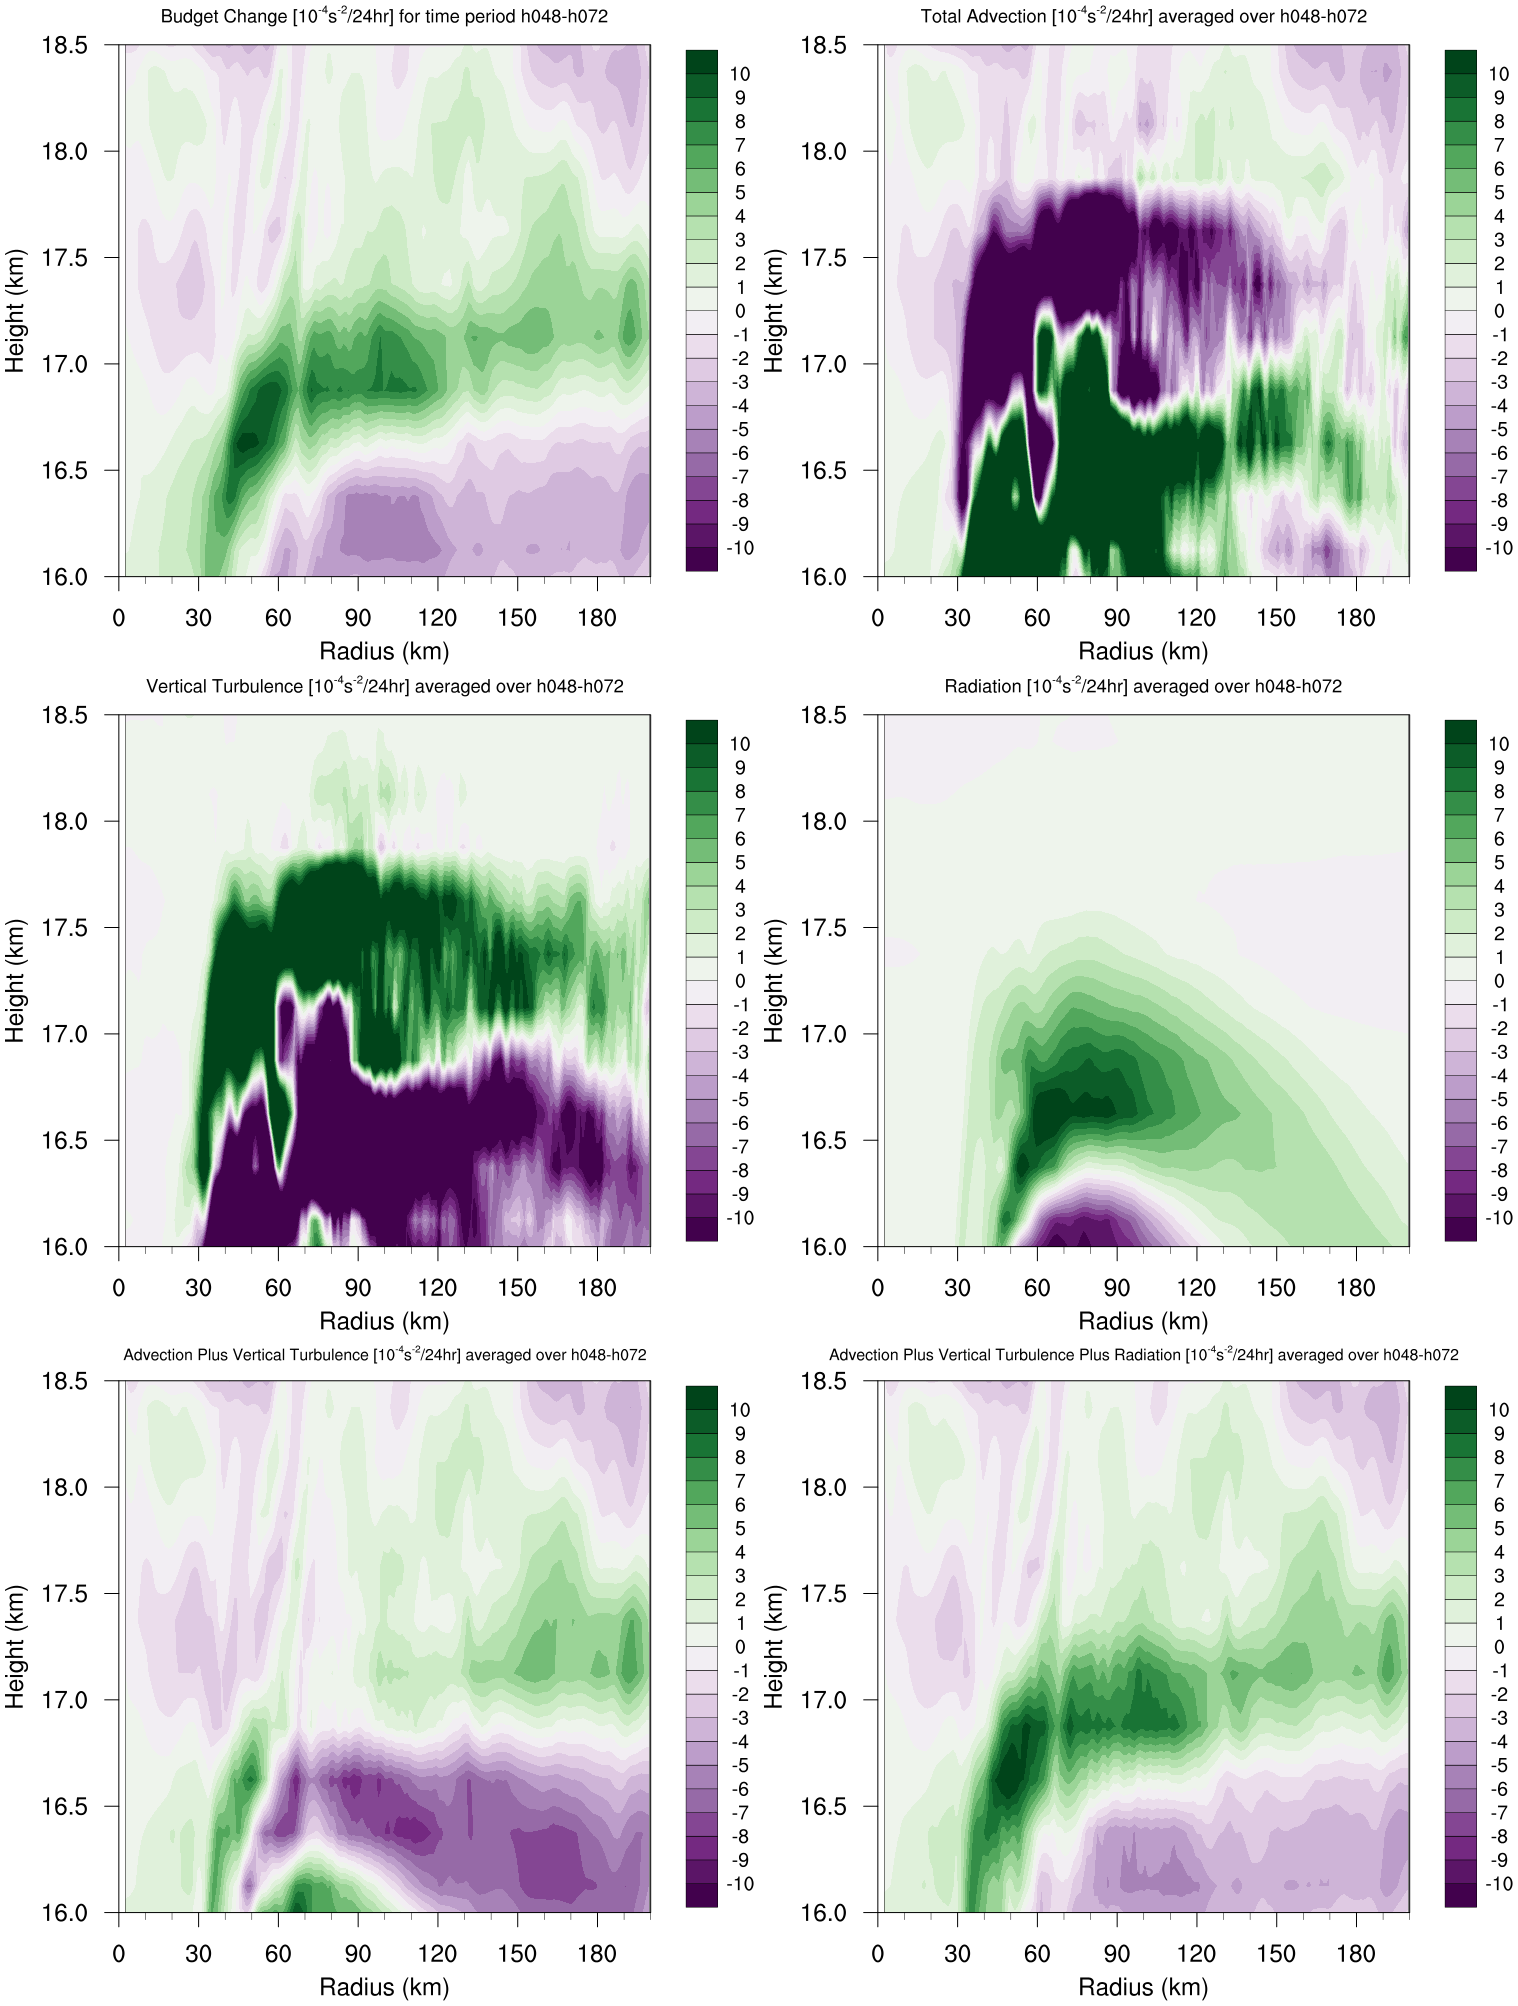
\includegraphics[width=39pc]{figures/fig07_h048-h072-budgetterms.png}}
\caption{}
\label{fig:48-72}
\end{figure*}

%FIGURE 8%
\begin{figure*}[ht]
\centerline{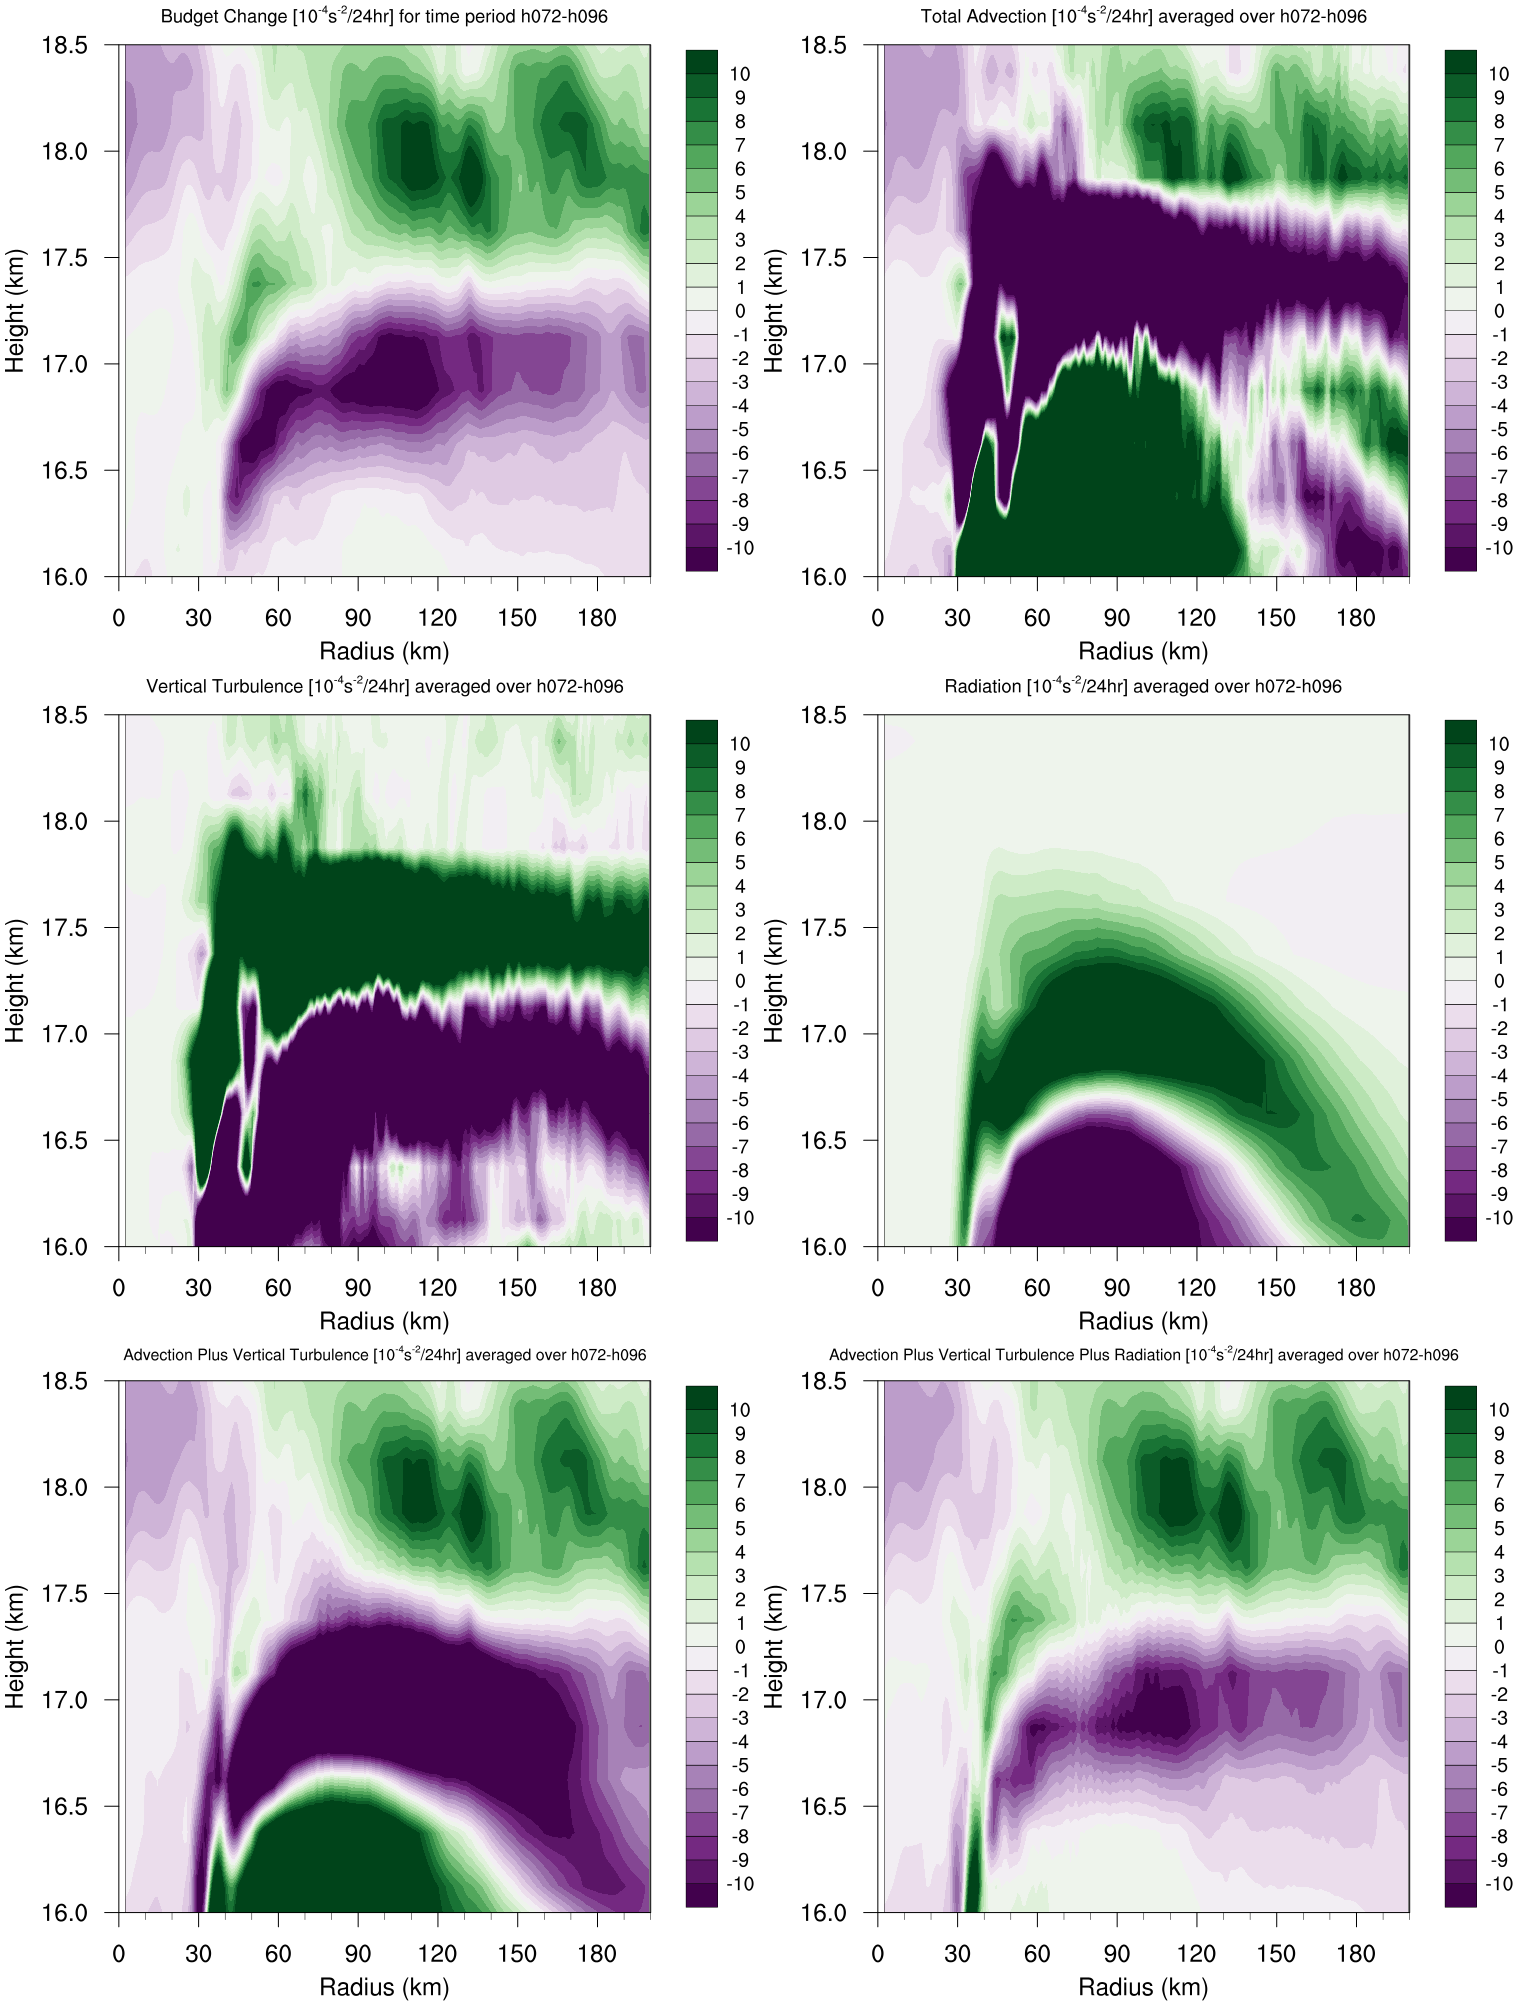
\includegraphics[width=39pc]{figures/fig08_h072-h096-budgetterms.png}}
\caption{}
\label{fig:72-96}
\end{figure*}

%\begin{figure}[t]
%  \noindent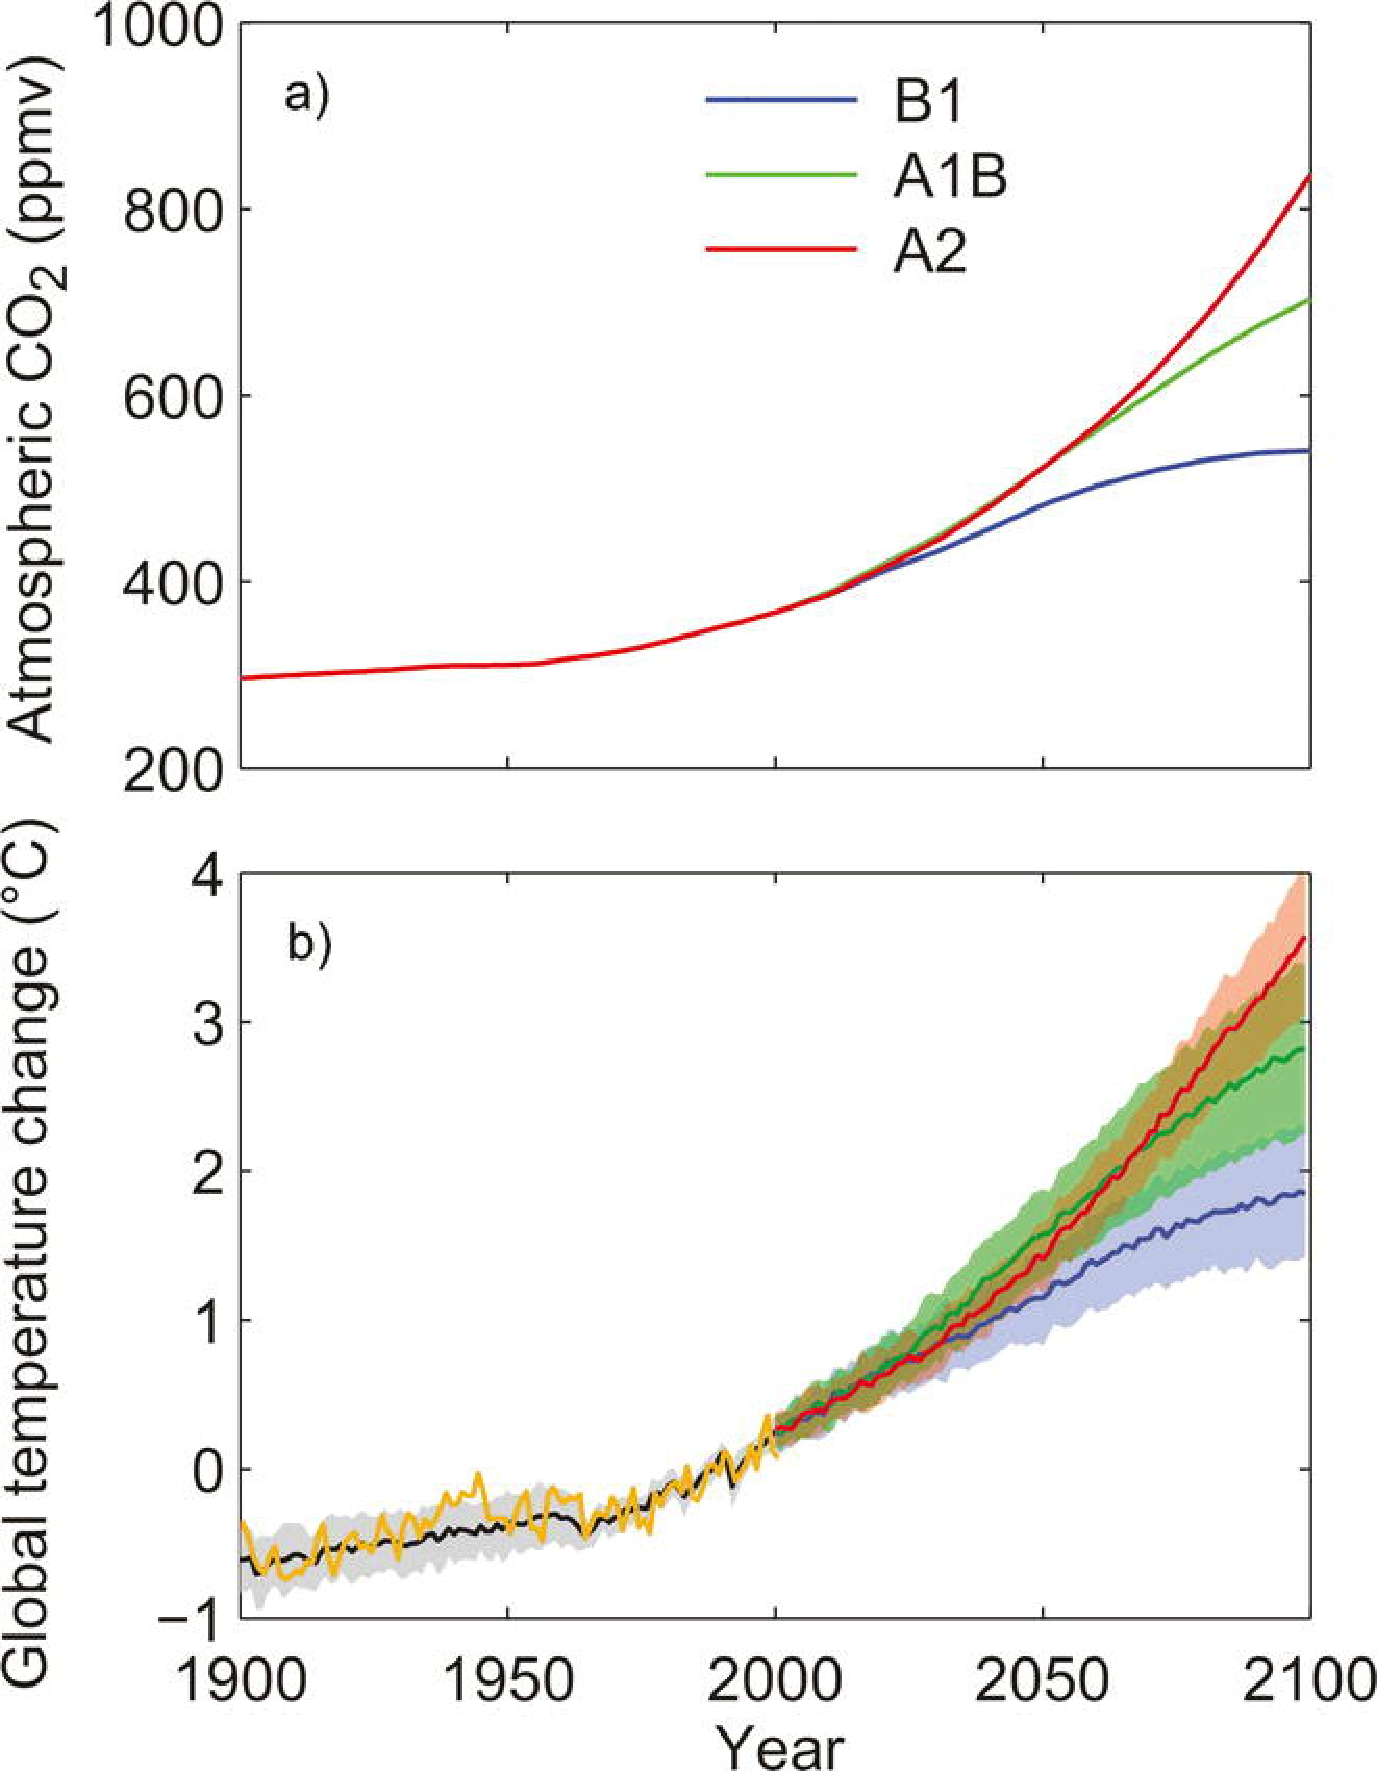
\includegraphics[width=19pc,angle=0]{figure01.pdf}\\
%  \caption{Enter the caption for your figure here.  Repeat as
%  necessary for each of your figures. Figure from \protect\cite{Knutti2008}.}\label{f1}
%\end{figure}

\end{document}
